% !TeX spellcheck = en_US

\documentclass{UTNetLab}

\title{Linux and TCP/IP Networking}
\newcommand\reference{
   S. Panwar, S. Mao, J.-dong Ryoo, and Y. Li, “Linux and TCP/IP networking,” in TCP/IP Essentials: A Lab-Based Approach, Cambridge: Cambridge University Press, 2004, pp. 26–42.
}

\begin{document}
	
	
\subsection{ Review and Guidance}
To use the prepared topology in PNETLab:
\begin{enumerate}
    \item In the directory of the corresponding experiment, open the required figure:
    \begin{figure}[H]
	\centering
	{\selectlanguage{english}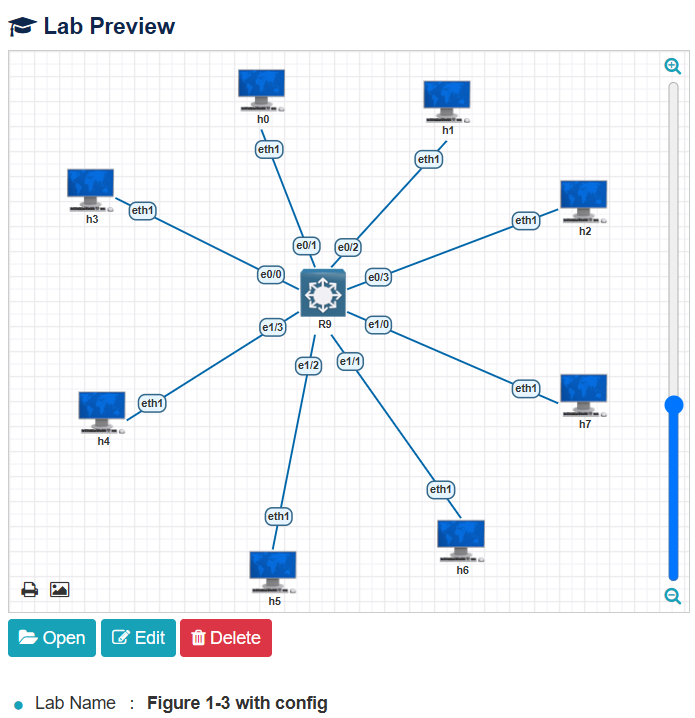
\includegraphics[scale=0.8]{img/1.png}}
	\caption{}
	\label{p01}
    \end{figure}
    
    \item From the \texttt{Left Panel}, in the \texttt{Setup Nodes} section, click on \texttt{Start All Nodes} to start all devices (or click on the triangular button of each device to start it):
    \begin{figure}[H]
	\centering
	{\selectlanguage{english}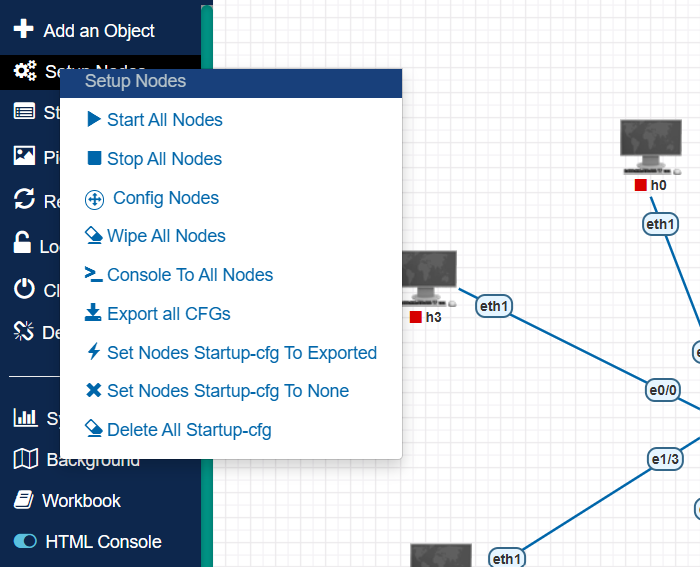
\includegraphics[scale=0.7]{img/2.png}}
	\caption{}
	\label{p02}
    \end{figure}

    \item Double click on each device to open its console:
    \begin{figure}[H]
	\centering
	{\selectlanguage{english}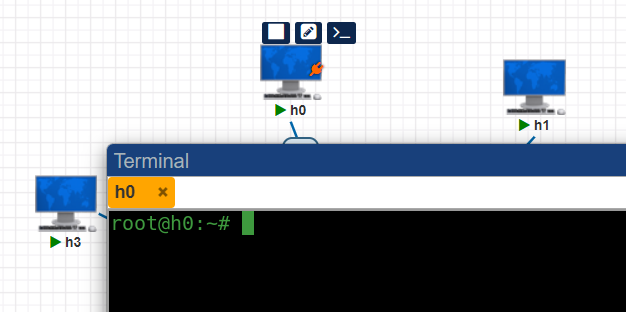
\includegraphics[scale=0.7]{img/3.png}}
	\caption{}
	\label{p03}
    \end{figure}
    
\end{enumerate}
    

\subsection{Attention}
You don't need to set IP addresses for each host in all figures prepared in PNETLab, because the IP addresses are set by default for all hosts. However, if you want to set the IP address for a host, you can open the console terminal by double-clicking on the host and typing the following command. For example, we set the IP address for host \lstinline{h0}.

\fcolorbox{blue}{green!10}{ {h\textsubscript{0}}'s Console }
\lstset{backgroundcolor=\color{green!10}}
\begin{lstlisting}
    ip address add 128.238.66.100/24 dev eth1
\end{lstlisting}


\subsection{Tips}
\fcolorbox{blue}{red!10}{h\textsubscript{0}'s Console}
\lstset{backgroundcolor=\color{red!10}}
\begin{lstlisting}
    ifconfig -a
\end{lstlisting}

This box means that, Double-click on host \textit{h0} to open its console terminal and type (run) this command in it:

\begin{figure}[H]
    \centering
    {\selectlanguage{english}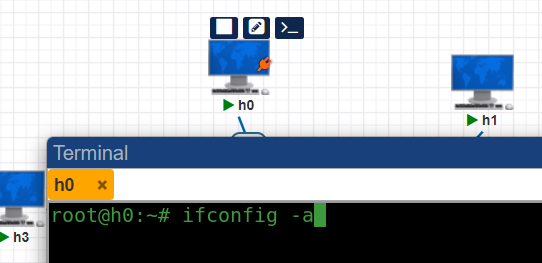
\includegraphics[scale=0.7]{img/4.png}}
    \caption{}
    \label{p04}
\end{figure}

\newpage

\section*{Objectives}
\begin{itemize}
    \item Getting acquainted with the lab environment.
    \item Getting acquainted with the Linux operating system.
    \item Preview of some TCP/IP diagnostic tools.
    \item Capturing and analyzing the link layer, IP, and TCP headers.
    \item Understanding the concept of encapsulation.
    \item Understanding the concept of multiplexing using \textit{port numbers}, the IP \textit{protocol} field, and the Ethernet \textit{frame type} field.
    \item Understanding the client–server architecture.
\end{itemize}

\part{Systems Configuration}
Launch PNETLab and make a network as below.
You can use \lstinline[emph={eth0}]{ifconfig eth1 192.168.0.1 netmask 255.255.255.0} to set ip.
\begin{center}
    \begin{minipage}{0.48\textwidth}
        \begin{flushleft}
            \begin{table}[H]
                \caption{The IP addresses of the hosts (Table~1.2)}
                \centering
                \begin{tabular}{ c c c }
                    \hline \hline
                    Host & IP Address     & Subnet Mask   \\
                    \hline
                    h0   & 128.238.66.100 & 255.255.255.0 \\
                    h1   & 128.238.66.101 & 255.255.255.0 \\
                    h2   & 128.238.66.102 & 255.255.255.0 \\
                    h3   & 128.238.66.103 & 255.255.255.0 \\
                    h4   & 128.238.66.104 & 255.255.255.0 \\
                    h5   & 128.238.66.105 & 255.255.255.0 \\
                    h6   & 128.238.66.106 & 255.255.255.0 \\
                    h7   & 128.238.66.107 & 255.255.255.0 \\
                    \hline \hline
                \end{tabular}
            \end{table}
        \end{flushleft}
    \end{minipage}
    \begin{minipage}{0.48\textwidth}
        \begin{flushright}
            \begin{figure}[H]
                \centering
                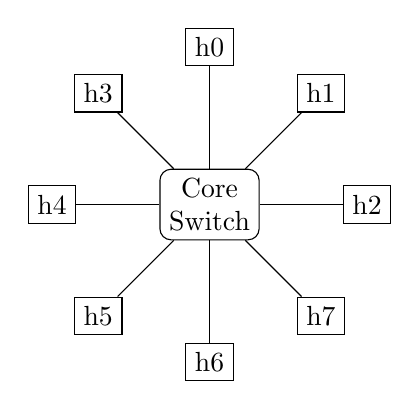
\begin{tikzpicture}
                    \node[draw,align=center,rounded corners] (s) at (0,0){Core\\Switch};
                    \node[draw] (h0) at (0,2){h0};
                    \node[draw] (h1) at ({sqrt(2)},{sqrt(2)}){h1};
                    \node[draw] (h2) at (2,0){h2};
                    \node[draw] (h3) at (-{sqrt(2)},{sqrt(2)}){h3};
                    \node[draw] (h4) at (-2,0){h4};
                    \node[draw] (h5) at (-{sqrt(2)},-{sqrt(2)}){h5};
                    \node[draw] (h6) at (0,-2){h6};
                    \node[draw] (h7) at ({sqrt(2)},-{sqrt(2)}){h7};

                    \draw (h0) -- (s);
                    \draw (h1) -- (s);
                    \draw (h2) -- (s);
                    \draw (h3) -- (s);
                    \draw (h4) -- (s);
                    \draw (h5) -- (s);
                    \draw (h6) -- (s);
                    \draw (h7) -- (s);
                \end{tikzpicture}
                \caption{A single segment network (Figure~1.3)}
            \end{figure}
        \end{flushright}
    \end{minipage}
\end{center}

\section{Telnet Service}
Run \lstinline{ps -e} to list the processes running in the \textit{h1}.

\fcolorbox{blue}{red!10}{h\textsubscript{1}'s Console}
\lstset{backgroundcolor=\color{red!10}}
\begin{lstlisting}
	ps -e
\end{lstlisting}

Start a new process by running \lstinline{telnet} in the background (adding an \lstinline{&} to the end of a command will run it in the background, and the \lstinline{fg} command will bring it back to the foreground):

\fcolorbox{blue}{blue!10}{ h\textsubscript{1}'s Console} 
\lstset{backgroundcolor=\color{blue!10}}
\begin{lstlisting}
	telnet &
\end{lstlisting}

Then execute \lstinline{ps -e} again to see if there is any change in its output.

\newpage
\fcolorbox{blue}{red!10}{h\textsubscript{1}'s Console}
\lstset{backgroundcolor=\color{red!10}}
\begin{lstlisting}
	ps -e
\end{lstlisting}

Find the process id of the \lstinline{telnet} process you started, by:

\fcolorbox{blue}{red!10}{h\textsubscript{1}'s Console}
\lstset{backgroundcolor=\color{red!10}}
\begin{lstlisting}
	ps -e | grep telnet
\end{lstlisting}

Then use \lstinline[emph={process-id-of-telnet}]{kill process-id-of-telnet} to terminate the \lstinline{telnet} process (you may need to run \lstinline{fg} to see its effect).

\begin{report}
    \item What is Internet Service Daemon (\lstinline{inetd})?

    \item Is \lstinline{inetd} started in your system? Why?

    \item Is \lstinline{xinetd} started in your system? What is its PID?
\end{report}

\section{Default Network Services}
Display the file \path{/etc/services} on the \textit{h1} screen, using:

\fcolorbox{blue}{red!10}{h\textsubscript{1}'s Console}
\lstset{backgroundcolor=\color{red!10}}
\begin{lstlisting}
	more /etc/services
\end{lstlisting}

Then in a background process, use the redirect operator to redirect the \lstinline{more} output to
a file using \lstinline{more /etc/services > ser-more}.

\fcolorbox{blue}{blue!10}{ h\textsubscript{1}'s Console} 
\lstset{backgroundcolor=\color{blue!10}}
\begin{lstlisting}
	more /etc/services > ser-more &
\end{lstlisting}

Compare the file \path{ser-more} with the original \lstinline{more} output in the command window.

Copy \path{/etc/services} file to a local file named \path{ser-cp} in your working directory (use \lstinline{pwd} to see working directory path),
using \lstinline{cp /etc/services ser-cp}.

\fcolorbox{blue}{red!10}{h\textsubscript{1}'s Console}
\lstset{backgroundcolor=\color{red!10}}
\begin{lstlisting}
	cp /etc/services ser-cp
\end{lstlisting}

Compare files \path{ser-more} and \path{ser-cp}, using \lstinline{cmp ser-more ser-cp}.
Are these two files identical?

\fcolorbox{blue}{red!10}{h\textsubscript{1}'s Console}
\lstset{backgroundcolor=\color{red!10}}
\begin{lstlisting}
	cmp ser-more ser-cp
\end{lstlisting}

Concatenate these two files using \lstinline{cat ser-more ser-cp > ser-cat}.

\fcolorbox{blue}{red!10}{h\textsubscript{1}'s Console}
\lstset{backgroundcolor=\color{red!10}}
\begin{lstlisting}
	cat ser-more ser-cp > ser-cat
\end{lstlisting}

Display the file sizes using \lstinline{ls -l ser*}.
Save the output.

\fcolorbox{blue}{red!10}{h\textsubscript{1}'s Console}
\lstset{backgroundcolor=\color{red!10}}
\begin{lstlisting}
	ls -l ser*
\end{lstlisting}

\begin{report}
    \item What are the sizes of files \path{ser-more}, \path{ser-cp}, and \path{ser-cat}?
\end{report}

\section{Network Command Manual}
Read the \lstinline{man} pages for the following programs:
\begin{multicols}{3}
    \begin{enumerate}
        \item \lstinline{arp}
        \item \lstinline{arping}
        \item \lstinline{ifconfig}
        \item \lstinline{tcpdump}
        \item \lstinline{ping}
        \item \lstinline{netstat}
        \item \lstinline{route}
        \item \lstinline{wireshark}
        \item \lstinline{iptables}
    \end{enumerate}
\end{multicols}

For example,  run the following command:

\fcolorbox{blue}{red!10}{h\textsubscript{1}'s Console}
\lstset{backgroundcolor=\color{red!10}}
\begin{lstlisting}
	man arp
\end{lstlisting}

Study the different options associated with each command.
Throughout this lab, you will use these commands rather extensively.

\begin{report}
    \item Explain the above commands briefly.
    (Two or three sentences per command would be adequate.)
\end{report}

\section{Packet Capturing}
In this exercise, we will use \lstinline{tcpdump} or \lstinline{wireshark} to capture a packet containing the link, IP, and TCP headers and analyze this packet.

\textit{Note:} In PNETLab you can capture and see a packet in \lstinline{wireshark} by right-clicking on a network device and selecting \textit{Capture} (usually on \texttt{eth1} interface).

First, run \lstinline{wireshark} on the \texttt{eth1} interface of \textit{h1} (or you can run \lstinline{tcpdump} in a secondary console).

Then, you may want to run \lstinline{telnet 128.238.66.102} in the \textit{h1} to generate some TCP traffic.\footnote{Remember to run \lstinline{/etc/init.d/xinetd restart} in the \textit{h2} to start telnet server on it.}

\fcolorbox{blue}{red!10}{h\textsubscript{1}'s Console}
\lstset{backgroundcolor=\color{red!10}}
\begin{lstlisting}
	telnet 128.238.66.102
\end{lstlisting}

After you login to \textit{h2} (\textit{Note:} use \textbf{netlab} for username and password), terminate the \lstinline{telnet} session (press \textit{CTRL+D} or run \textit{kill} command) and stop capturing in \lstinline{wireshark} (click on \textit{stop capturing packets} red square button in the toolbar).


Now, you will see the packet trace captured by \lstinline{wireshark} (or \lstinline{tcpdump}) and analyze the captured packets. Select any one of the packets that contain the link, IP, and TCP headers.


\begin{report}
    \item What is the value of the \texttt{protocol} field in the IP header of the packet you saved?
    What is the use of the \texttt{protocol} field?

    \item What is the value of the \texttt{frame type} field in an Ethernet frame carrying an IP datagram?
\end{report}

\section{\texttt{ARPing}}
This time we will run \lstinline{wireshark} to capture an ARP request and an ARP reply in real-time.
Simply run \lstinline{wireshark} on the \textit{h1} with right click and select \textbf{capture} item on \texttt{eth1} interface to start capturing\footnote{On physical machine, can start capture with \lstinline{wireshark &} command.}.
If there are no arp requests and replies in the network, generate some using the \lstinline{arping 128.238.66.102} command in the \textit{h1} terminal.

\fcolorbox{blue}{red!10}{h\textsubscript{1}'s Console}
\lstset{backgroundcolor=\color{red!10}}
\begin{lstlisting}
	arping 128.238.66.102
\end{lstlisting}

Now you should see several ARP replies in the \lstinline{arping} output.

\begin{report}
    \item What is the value of the \texttt{frame type} field in an Ethernet frame carrying an ARP request and in an Ethernet frame carrying an ARP reply, respectively?

    \item What is the use of the \texttt{frame type} field?
\end{report}

\section{Packet Filtering}
Using the \lstinline{wireshark} or \lstinline{tcpdump} utilities, capture any packet on the LAN and see the output format for different filtering options.
Study the various expressions for selecting which packets to be dumped.

For this experiment, use the \lstinline{man} page for \lstinline{tcpdump} to find out the options and expressions that can be used.

If there is no traffic on the network, you may generate traffic with some applications (e.g. \lstinline{telnet}, \lstinline{ping}, etc.).

\begin{report}
    \item Explain briefly the purposes of the following \lstinline{tcpdump} expressions.
\end{report}

% todo: make sample traffic
If you are using \lstinline{tcpdump}, explain the following filters:
\begin{itemize}
    \item \lstinline{tcpdump udp port 520}
    \item \lstinline{tcpdump -x -s 120 ip proto 89}
    \item \lstinline[emph={ip-addr1, ip-addr2, ip-addr3}]{tcpdump -x -s 70 host ip-addr1 and (ip-addr2 or ip-addr3)}
    \item \lstinline[emph={ip-addr1, ip-addr2}]{tcpdump -x -s 70 host ip-addr1 and not ip-addr2}
\end{itemize}

If you are using \lstinline{wireshark} explain the following filters:
\begin{itemize}
    \item \lstinline{udp.port == 520}
    \item \lstinline{ip.proto == 89}
    \item \lstinline[emph={ip-addr1, ip-addr2, ip-addr3}]{ip.addr == ip-addr1 and (ip.addr == ip-addr2 or ip.addr == ip-addr3)}
    \item \lstinline[emph={ip-addr1, ip-addr2}]{ip.addr == ip-addr1 and not ip.addr ip-addr2}
\end{itemize}

\section{Connection Port}
Run \lstinline{wireshark} on the \texttt{eth1} interface of the \textit{h1}.

Then execute a TCP utility, \lstinline{telnet} for example, in command window:

\fcolorbox{blue}{red!10}{h\textsubscript{1}'s Console}
\lstset{backgroundcolor=\color{red!10}}
\begin{lstlisting}
	telnet 128.238.66.102
\end{lstlisting}


\begin{report}
    \item What are the port numbers used by the \textit{h1} (local machine) and the \textit{h2} (remote machine)?

    \item Which port numbers matches the port number listed for \lstinline{telnet} in the \path{/etc/services} file?
\end{report}


\section{Random Port}
Run \lstinline{wireshark} on the \texttt{eth1} interface of the \textit{h1}.

Now, \lstinline{telnet} to the \textit{h2}, one from a background session by typing \lstinline{telnet 128.238.66.102 &}.

\fcolorbox{blue}{blue!10}{ h\textsubscript{1}'s Console} 
\lstset{backgroundcolor=\color{blue!10}}
\begin{lstlisting}
	telnet 128.238.66.102 &
\end{lstlisting}

Then, open another \lstinline{telnet} session to the \textit{h2} in the foreground by typing \lstinline{telnet 128.238.66.102}.

\fcolorbox{blue}{red!10}{h\textsubscript{1}'s Console}
\lstset{backgroundcolor=\color{red!10}}
\begin{lstlisting}
	telnet 128.238.66.102
\end{lstlisting}

Now you are opening two \lstinline{telnet} sessions to \textit{h2} simultaneously, one in the background and another in the foreground.
% On each telnet terminal, run \lstinline{pwd} to generate traffic.

Check the port numbers being used on both sides of the two connections from the output in the \lstinline{wireshark} window.

\begin{report}
    \item When you have two \lstinline{telnet} sessions with your machine, what port number is used on the \textit{h2} (remote machine)?

    \item Are both sessions connected to the same port number on the \textit{h2} (remote machine)?

    \item What port numbers are used in the \textit{h1} (local machine) for the first and second \lstinline{telnet}, respectively?

    \item Explain briefly what a \lstinline{socket} is.
\end{report}
\end{document}